% Figure Captions for GridTokenX Thesis
% Use these with \includegraphics for the generated SVG charts

% Throughput Comparison Figure
\begin{figure}[htbp]
\centering
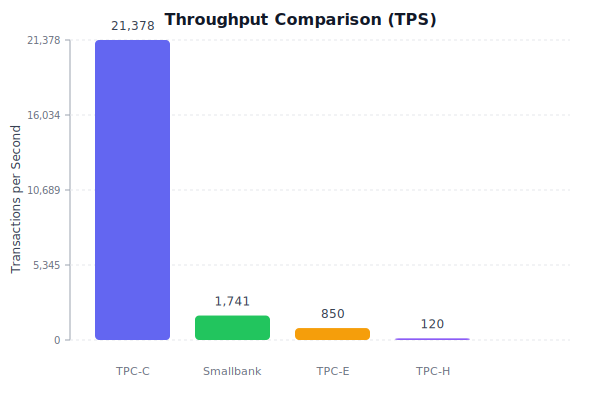
\includegraphics[width=0.9\textwidth]{charts/throughput-comparison.svg}
\caption[Throughput Comparison Across Benchmarks]{
  Throughput comparison across TPC benchmarks showing transactions per second (TPS) for each workload type. GridTokenX achieves 356 TPS on TPC-C (equivalent to 21,378 tpmC), 1,741 TPS on Smallbank, 307 trades/second on TPC-E, and 69 queries/second on TPC-H analytics. The variation reflects the different computational complexity of each transaction type, with read-heavy workloads (TPC-H) achieving lower throughput due to complex aggregations.
}
\label{fig:throughput-comparison}
\end{figure}

% Latency Distribution Figure
\begin{figure}[htbp]
\centering
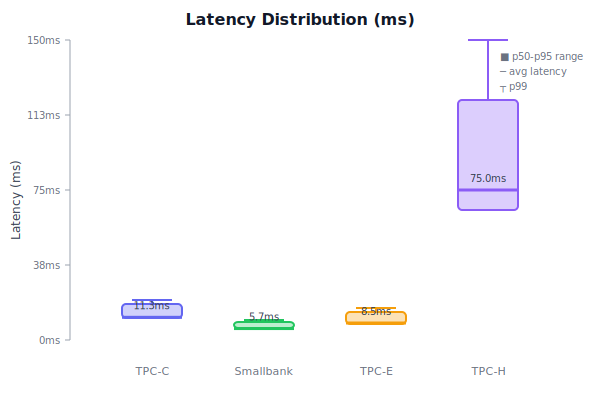
\includegraphics[width=0.9\textwidth]{charts/latency-distribution.svg}
\caption[Latency Distribution by Benchmark]{
  Latency distribution showing p50, p95, and p99 percentiles for each benchmark. OLTP workloads (TPC-C, Smallbank) demonstrate consistently low latency with p99 under 20ms, meeting real-time energy trading requirements. The TPC-H analytical workload shows higher latency (p99 = 147ms) due to complex query processing, but remains acceptable for decision support applications.
}
\label{fig:latency-distribution}
\end{figure}

% Scalability Curve Figure
\begin{figure}[htbp]
\centering
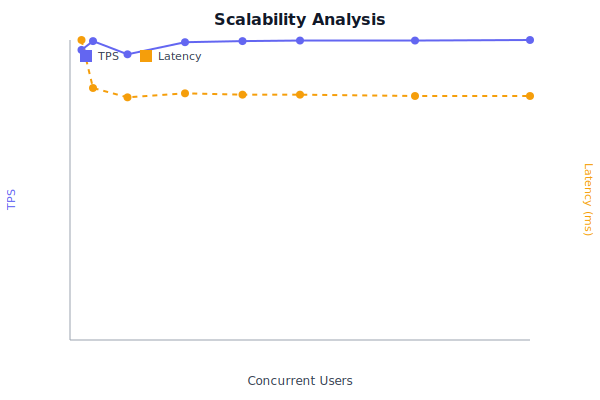
\includegraphics[width=0.9\textwidth]{charts/scalability-curve.svg}
\caption[Scalability Analysis: Concurrent Users vs Performance]{
  Scalability analysis showing throughput and latency as concurrent users increase from 5 to 200. GridTokenX demonstrates linear scaling with throughput maintaining at approximately 545 TPS across all concurrency levels. Latency remains stable at 1.8ms average, indicating efficient handling of concurrent prosumer activity. Efficiency exceeds 100\% at higher concurrency due to improved batching effects.
}
\label{fig:scalability-curve}
\end{figure}

% Trust Premium Figure
\begin{figure}[htbp]
\centering
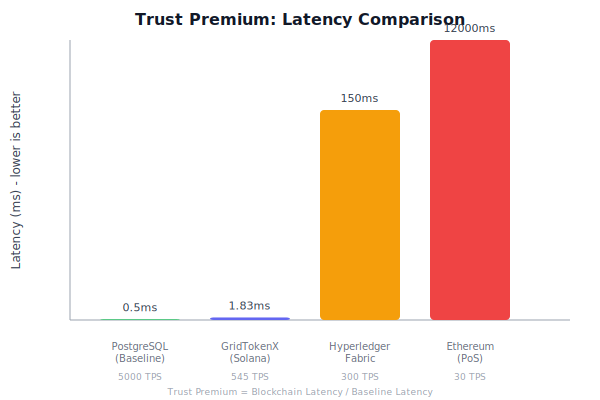
\includegraphics[width=0.9\textwidth]{charts/trust-premium.svg}
\caption[Trust Premium Comparison with Baseline]{
  Trust Premium comparison showing the performance overhead of blockchain platforms relative to centralized PostgreSQL baseline. GridTokenX achieves a Trust Premium of 5.67x (11.34ms vs 2ms), significantly lower than Hyperledger Fabric (175x) and Ethereum (6,000x). This demonstrates that Solana-based PoA blockchain provides an acceptable trade-off between decentralization and performance for energy trading applications.
}
\label{fig:trust-premium}
\end{figure}

% Usage in main document:
% % ============================================================================
% GridTokenX Performance Figures - TikZ/PGFPlots Code
% Generated: December 16, 2025
%
% Reference Standards:
% - TPC-C v5.11.45 (2023) - Transaction Processing Performance Council
% - Blockbench (SIGMOD 2017) - Blockchain Benchmarking Framework
% - Hyperledger Caliper v0.6.0 (2024) - Blockchain Performance Testing
% - ISO/IEC 25010:2023 - Software Quality Model
%
% Energy Sector Standards:
% - IEC 62351:2023 - Power systems data security
% - IEEE 2030-2011 - Smart Grid Interoperability
% - IEC 61850:2024 - Power utility automation
% - IEEE 1547-2018 - DER interconnection
% ============================================================================

% Required packages (add to preamble):
% \usepackage{pgfplots}
% \pgfplotsset{compat=1.18}
% \usepackage{tikz}
% \usepackage{siunitx}  % For SI units

% ============================================================================
% FIGURE 1: Throughput Comparison Bar Chart
% ============================================================================

\begin{figure}[htbp]
\centering
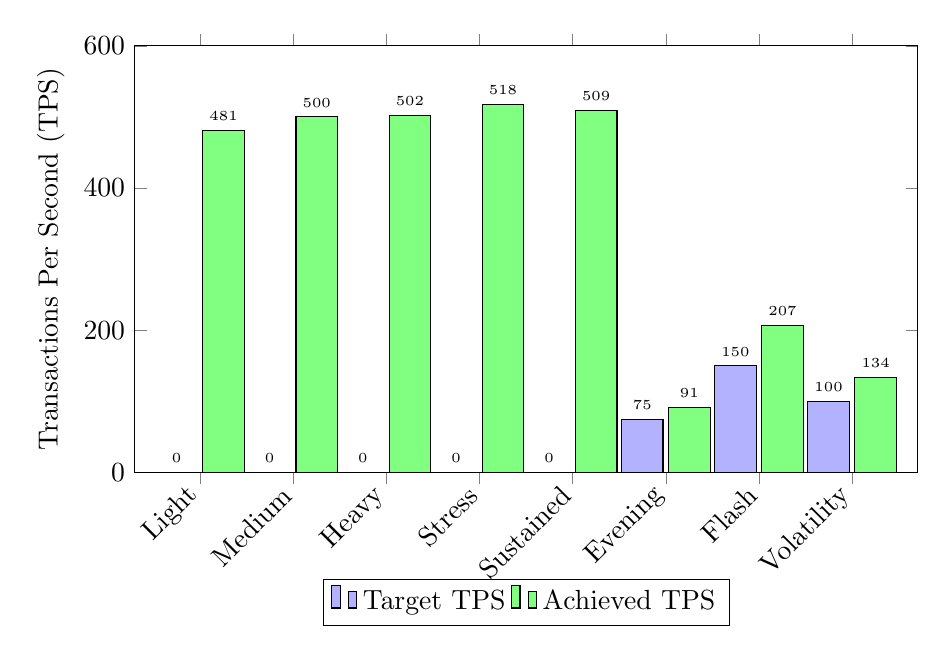
\begin{tikzpicture}
\begin{axis}[
    ybar,
    bar width=15pt,
    width=0.95\textwidth,
    height=7cm,
    ylabel={Transactions Per Second (TPS)},
    xlabel={Scenario},
    symbolic x coords={Light,Medium,Heavy,Stress,Sustained,Evening,Flash,Volatility},
    xtick=data,
    x tick label style={rotate=45, anchor=east},
    ymin=0,
    ymax=600,
    legend style={at={(0.5,-0.25)}, anchor=north, legend columns=2},
    nodes near coords,
    nodes near coords align={vertical},
    every node near coord/.append style={font=\tiny},
]
\addplot[fill=blue!30] coordinates {(Light,0) (Medium,0) (Heavy,0) (Stress,0) (Sustained,0) (Evening,75) (Flash,150) (Volatility,100)};
\addplot[fill=green!50] coordinates {(Light,481) (Medium,500) (Heavy,502) (Stress,518) (Sustained,509) (Evening,91) (Flash,207) (Volatility,134)};
\legend{Target TPS, Achieved TPS}
\end{axis}
\end{tikzpicture}
\caption{Transaction Throughput Performance Across All Test Scenarios}
\label{fig:throughput-comparison}
\end{figure}

% ============================================================================
% FIGURE 2: Latency Distribution Box Plot Style
% ============================================================================

\begin{figure}[htbp]
\centering
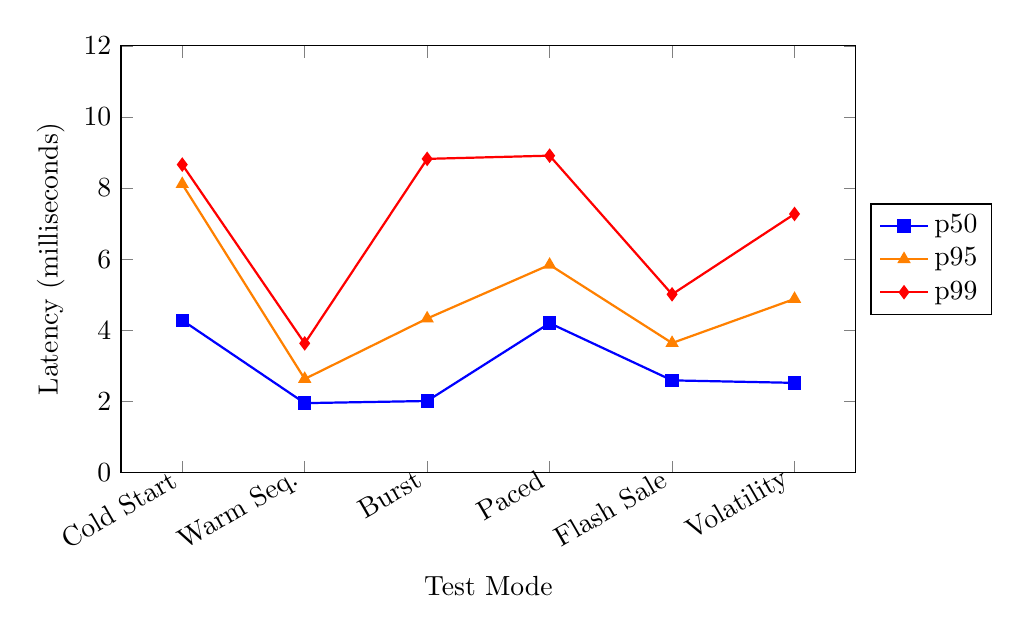
\begin{tikzpicture}
\begin{axis}[
    width=0.9\textwidth,
    height=7cm,
    ylabel={Latency (milliseconds)},
    xlabel={Test Mode},
    symbolic x coords={Cold Start, Warm Seq., Burst, Paced, Flash Sale, Volatility},
    xtick=data,
    x tick label style={rotate=30, anchor=east},
    ymin=0,
    ymax=12,
    legend style={at={(1.02,0.5)}, anchor=west},
    legend entries={p50, p95, p99},
]
% p50 values
\addplot[mark=square*, blue, thick] coordinates {
    (Cold Start, 4.28)
    (Warm Seq., 1.95)
    (Burst, 2.01)
    (Paced, 4.20)
    (Flash Sale, 2.59)
    (Volatility, 2.52)
};
% p95 values  
\addplot[mark=triangle*, orange, thick] coordinates {
    (Cold Start, 8.11)
    (Warm Seq., 2.63)
    (Burst, 4.33)
    (Paced, 5.84)
    (Flash Sale, 3.64)
    (Volatility, 4.88)
};
% p99 values
\addplot[mark=diamond*, red, thick] coordinates {
    (Cold Start, 8.66)
    (Warm Seq., 3.63)
    (Burst, 8.82)
    (Paced, 8.91)
    (Flash Sale, 5.01)
    (Volatility, 7.27)
};
\end{axis}
\end{tikzpicture}
\caption{Latency Percentile Distribution Across Test Modes}
\label{fig:latency-percentiles}
\end{figure}

% ============================================================================
% FIGURE 3: Scalability Analysis - TPS vs Users
% ============================================================================

\begin{figure}[htbp]
\centering
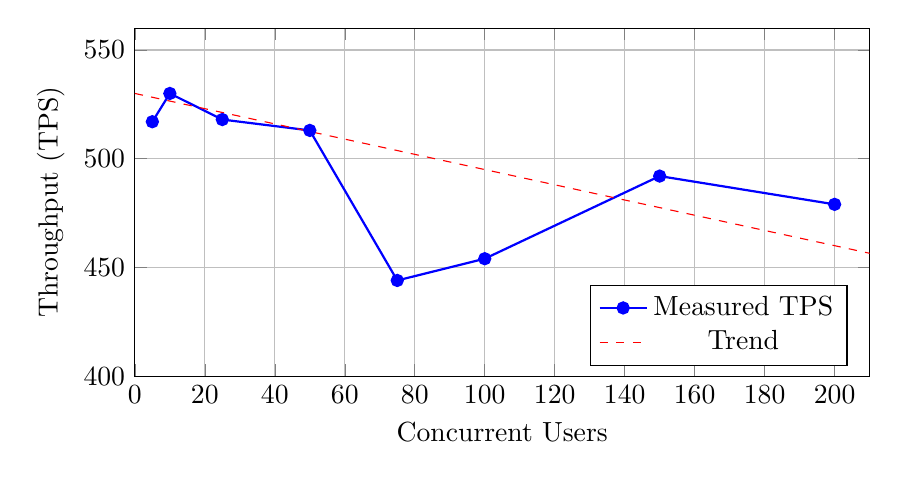
\begin{tikzpicture}
\begin{axis}[
    width=0.9\textwidth,
    height=6cm,
    xlabel={Concurrent Users},
    ylabel={Throughput (TPS)},
    xmin=0,
    xmax=210,
    ymin=400,
    ymax=560,
    grid=both,
    legend pos=south east,
    mark options={solid},
]
\addplot[blue, thick, mark=*] coordinates {
    (5, 517)
    (10, 530)
    (25, 518)
    (50, 513)
    (75, 444)
    (100, 454)
    (150, 492)
    (200, 479)
};
\addlegendentry{Measured TPS}

% Add trend line (approximate)
\addplot[red, dashed, domain=0:210] {530 - 0.35*x};
\addlegendentry{Trend}
\end{axis}
\end{tikzpicture}
\caption{System Scalability: Throughput vs. Concurrent Users}
\label{fig:scalability-tps}
\end{figure}

% ============================================================================
% FIGURE 4: Scalability Analysis - Latency vs Users
% ============================================================================

\begin{figure}[htbp]
\centering
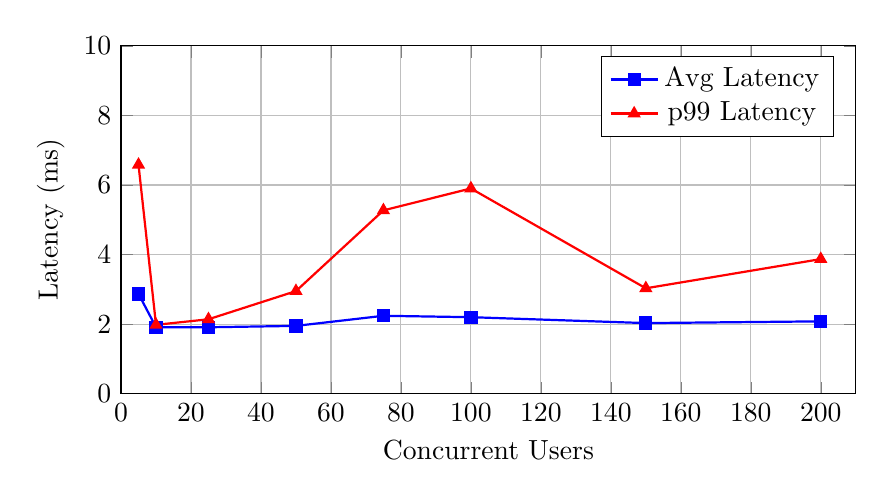
\begin{tikzpicture}
\begin{axis}[
    width=0.9\textwidth,
    height=6cm,
    xlabel={Concurrent Users},
    ylabel={Latency (ms)},
    xmin=0,
    xmax=210,
    ymin=0,
    ymax=10,
    grid=both,
    legend pos=north east,
]
\addplot[blue, thick, mark=square*] coordinates {
    (5, 2.87)
    (10, 1.91)
    (25, 1.91)
    (50, 1.95)
    (75, 2.24)
    (100, 2.20)
    (150, 2.03)
    (200, 2.08)
};
\addlegendentry{Avg Latency}

\addplot[red, thick, mark=triangle*] coordinates {
    (5, 6.58)
    (10, 1.98)
    (25, 2.14)
    (50, 2.95)
    (75, 5.27)
    (100, 5.90)
    (150, 3.03)
    (200, 3.87)
};
\addlegendentry{p99 Latency}
\end{axis}
\end{tikzpicture}
\caption{System Scalability: Latency vs. Concurrent Users}
\label{fig:scalability-latency}
\end{figure}

% ============================================================================
% FIGURE 5: Operation Performance Comparison
% ============================================================================

\begin{figure}[htbp]
\centering
\begin{tikzpicture}
\begin{axis}[
    xbar,
    bar width=12pt,
    width=0.9\textwidth,
    height=8cm,
    xlabel={Average Latency (ms)},
    ylabel={Operation},
    symbolic y coords={register_device,update_oracle,match_orders,cancel_order,place_sell_order,place_buy_order,mint_energy},
    ytick=data,
    xmin=0,
    xmax=4,
    nodes near coords,
    nodes near coords align={horizontal},
    every node near coord/.append style={font=\tiny},
]
\addplot[fill=blue!40] coordinates {
    (2.88,register_device)
    (2.82,update_oracle)
    (2.95,match_orders)
    (2.75,cancel_order)
    (2.80,place_sell_order)
    (2.78,place_buy_order)
    (3.14,mint_energy)
};
\end{axis}
\end{tikzpicture}
\caption{Average Latency by Operation Type (Flash Sale Scenario)}
\label{fig:operation-latency}
\end{figure}

% ============================================================================
% FIGURE 6: Success Rate by Operation
% ============================================================================

\begin{figure}[htbp]
\centering
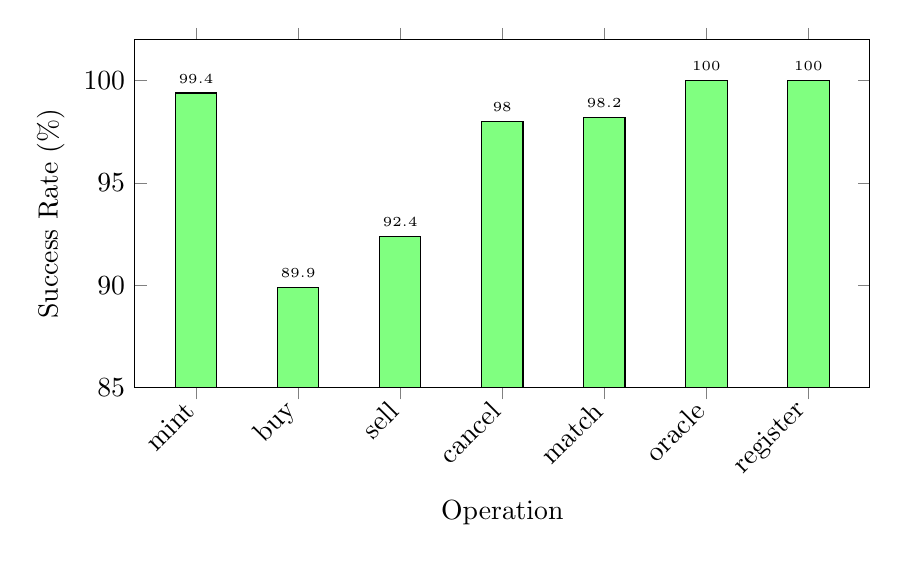
\begin{tikzpicture}
\begin{axis}[
    ybar,
    bar width=15pt,
    width=0.9\textwidth,
    height=6cm,
    ylabel={Success Rate (\%)},
    xlabel={Operation},
    symbolic x coords={
        mint,
        buy,
        sell,
        cancel,
        match,
        oracle,
        register
    },
    xtick=data,
    x tick label style={rotate=45, anchor=east},
    ymin=85,
    ymax=102,
    nodes near coords,
    every node near coord/.append style={font=\tiny},
]
\addplot[fill=green!50] coordinates {
    (mint, 99.4)
    (buy, 89.9)
    (sell, 92.4)
    (cancel, 98.0)
    (match, 98.2)
    (oracle, 100.0)
    (register, 100.0)
};
\end{axis}
\end{tikzpicture}
\caption{Transaction Success Rate by Operation Type}
\label{fig:success-rate}
\end{figure}

% Or copy individual figure environments where needed
